\section{Experiments}
\label{sec:experiments}

\subsection{Number of Iterations}
One of the major flaws in the graph net framework is the issue of determining how many iterations to run.
In theory, because of the universal approximation properties of neural nets, the optimal number of iterations is any number larger than the diameter of the graph, so that each node can make a fully informed decision knowing the entire graph topology.
However, this is not realistic: as shown in Figure~\ref{fig:dataset-graph-stats}, the maximum diameter of a given graph

\begin{figure}
  \centering
  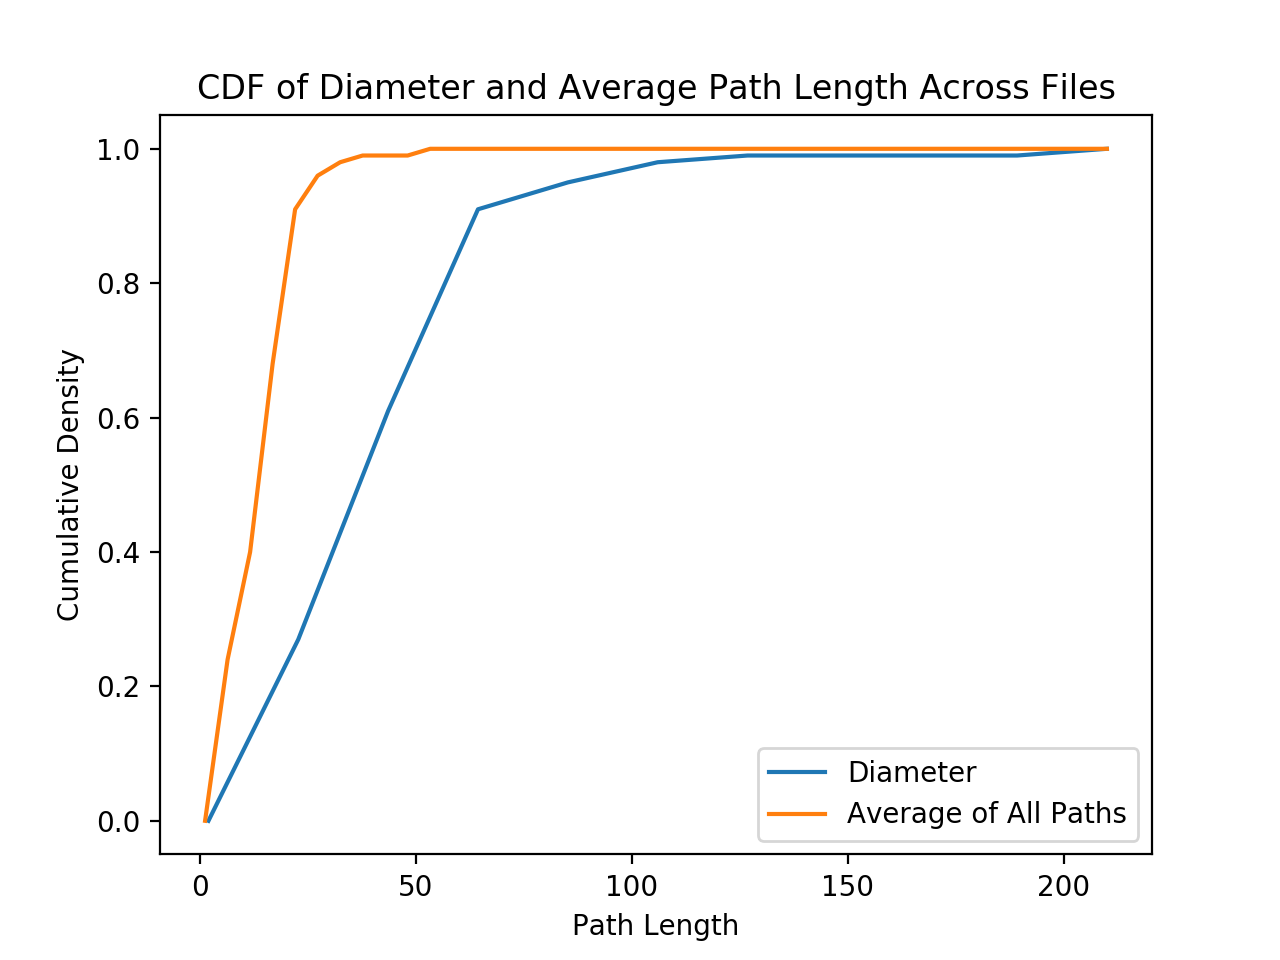
\includegraphics[width=\linewidth]{img/diameter}
  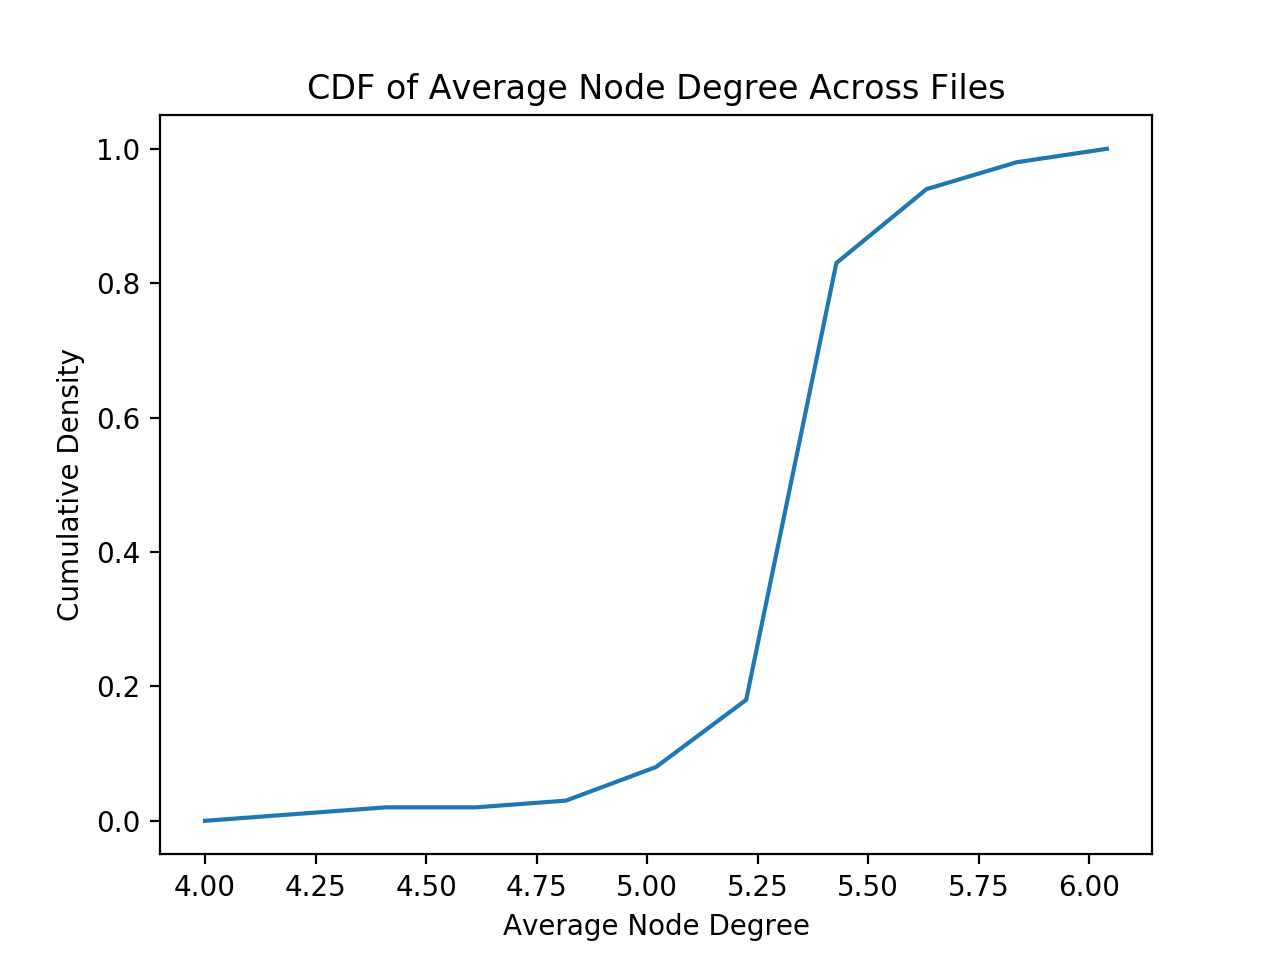
\includegraphics[width=\linewidth]{img/node_degree}
  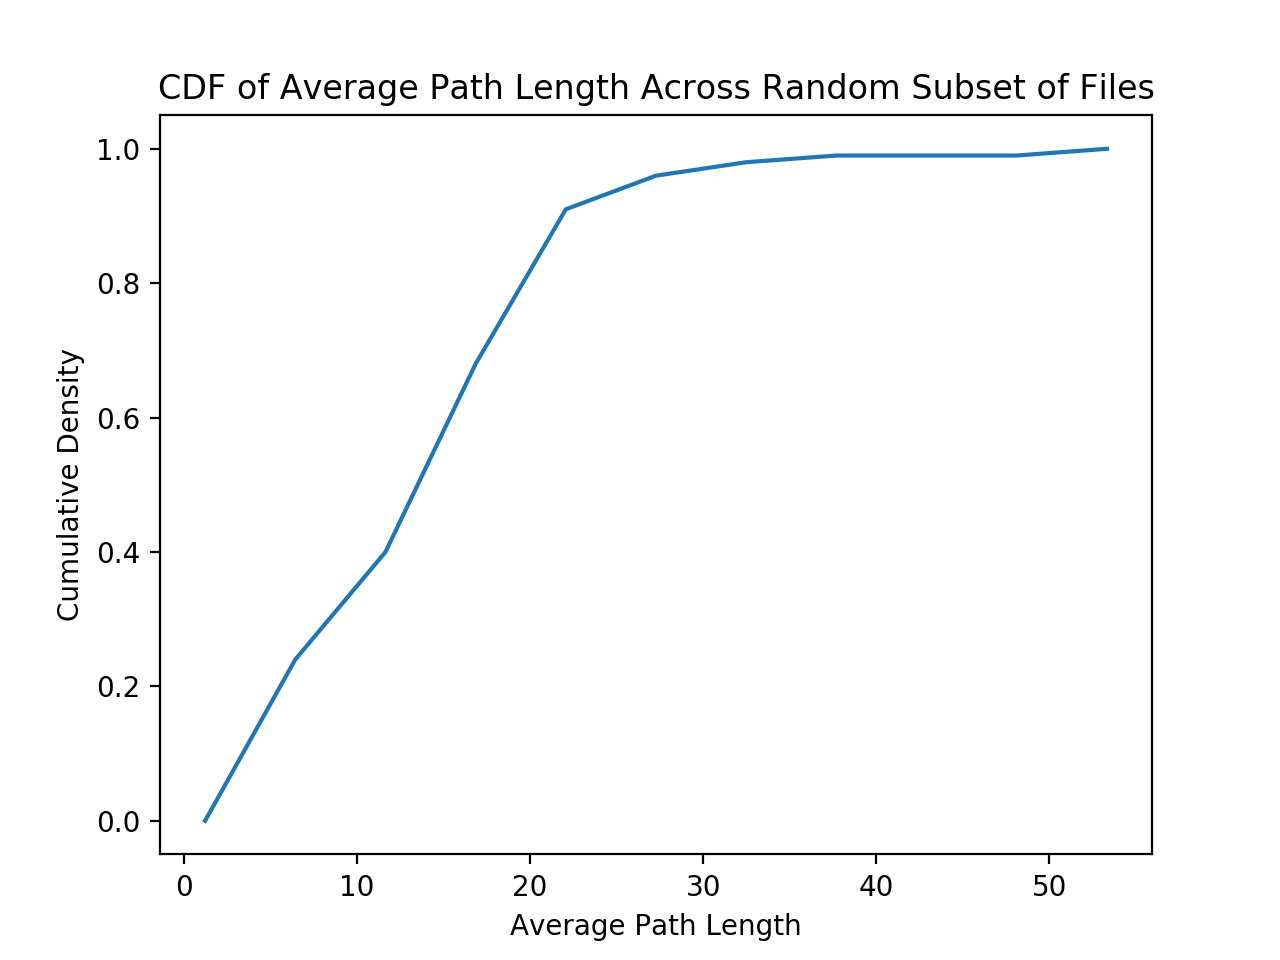
\includegraphics[width=\linewidth]{img/path_length}
  \caption{Foo}
  \label{fig:dataset-graph-stats}
\end{figure}


Graph nets do not have the same guarantee as other approximation

\paragraph{Iteration Ensemble.}

\paragraph{Bayesian Optimization.}

\subsection{Edge Ablation}

\todo{Experiments, Results}

%%% Local Variables:
%%% TeX-master: "main"
%%% End: